In this master thesis, 
a twin is defined as a pair of homologues found in the same organism,
but for which one is naturally located in the cytoplasm and the other in the periplasm.
Such twins often have similar structural and biophysical features,
but those that are different could be interesting in context of translocation.
It also allows to more closely examine the effect of signal peptides on the  biophysical landscape.

The goal of the pipeline described below (Fig. \ref{fig:twin_overview}) was to generate an extensive set of cytoplasm / periplasm twins.
This was achieved by combining the powerful annotation system of UniProtKB with standard bioinformatics tools.
To start, the query retrieval REST API was utilised to retrieve a set of cytoplasmic and periplasmic proteins, and the organisms they reside in. 
Multiple datasets were generated on different taxonomic levels ranging from the family of Enterobacteriaceae to the domain of all Bacteria.
Next, the proteins were clustered by organism and local BLAST search of cytoplasmic against periplasmic proteins was performed to identify homologues twins.
To look at the twins in an evolutionary relevant context,
more distant homologues were retrieved and two multiple sequence alignments were generated for each twin
(one for the cytoplasmic and one for the periplasmic protein).
Traditional methods to search for homologues such as BLAST (\cite{johnson2008})
and 
JackHMMer (\cite{johnson2010})
are to slow to use on large scale.
Additionally, I could not find an API to automate the process.
Therefore the UniProtKB mapping REST APA was utilised to obtain the UniRef50 clusters.
All members within a clusters have at least 50 percent sequence identity.
Subsequently, 
cd-hit (\cite{li2006}) clustered the UniRef50 members to a sequence identity threshold of 90 percent threshold to reduce sampling bias.
Finally, ClustalOmega (\cite{sievers2014}) generated a MSA from these members with at most 90 percent sequence identity.

~\begin{figure}[h!]
	~\begin{subfigure}[b]{\linewidth}
		\centering
		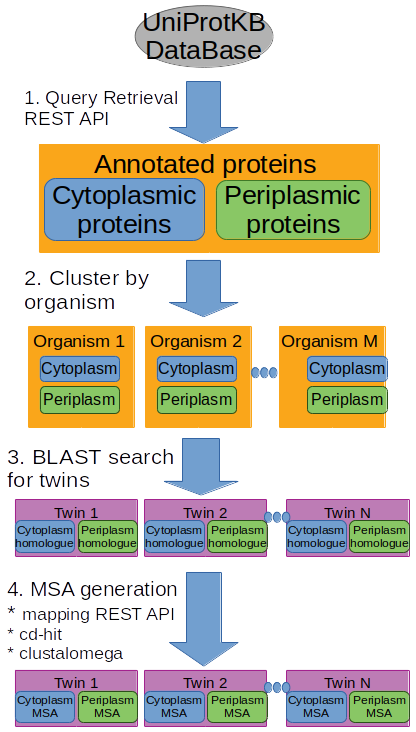
\includegraphics[width=\linewidth, height=0.6\textheight, keepaspectratio]
		{./methods/pipeline_twin_search/img/generalFigure.png}
	~\end{subfigure}
	\caption{
		\textbf{General overview of the cytoplasm / periplasm twin search.}
	}
	\label{fig:twin_overview}
~\end{figure}

